\documentclass[a4paper,answers]{exam}
\usepackage{graphicx} % Required for inserting images

\usepackage{amsmath}
\usepackage{amssymb}

\title{CS215 Assignment-1}
\author{Malay Kedia (Roll No. 23B1034) \\ Aakash Gupta (Roll No. 23B0953) \\ Yash Singh (Roll No. 23B0934)}
\date{}

\begin{document}
\maketitle

\begin{questions}


\question{\bf Normal Sampling}

Task A:
\begin{solution}
Consider the random variable \( Y := F_X(X) \) in \([0,1]\).

To find its distribution, we compute the CDF of \( Y \), denoted by \( F_Y(y) \). By definition:
   \[
   F_Y(y) = P(Y \leq y) = P(F_X(X) \leq y).
   \]

ATQ, \( F_X \) is invertible, ie, there exists a function \( F_X^{-1} \) which is inverse of $F_X$. 

Since \( Y = F_X(X) \), the event \( F_X(X) \leq y \) is equivalent to the event \( X \leq F_X^{-1}(y) \). Therefore, we have:
   \[
   F_Y(y) = P(X \leq F_X^{-1}(y)) = F_X(F_X^{-1}(y)) \hspace{1cm} \text{(by definition of CDF for X)}
   \]
   \[ \forall y \in [0, 1] \hspace{0.5cm} F_X(F_X^{-1}(y)) = y  \implies F_Y(y) = y.
   \]
The CDF of \( Y \) is \( F_Y(y) = y \) for \( y \in [0, 1] \), which is exactly the CDF of a uniformly distributed random variable on \([0, 1]\).

Thus, \( Y \) is uniformly distributed on \([0, 1]\).
\end{solution}

Task B:
\begin{solution}\\
Assumption: We know the CDF of X.\\
Given a random variable \( Y \) uniformly distributed over \([0,1]\), an algorithm \( \mathcal{A} \) that transforms Y into a sample from a random variable with the CDF of \( X \) can be constructed as follows:

Let \( Y \sim \text{Uniform}(0,1) \). Suppose \( F_X \) is the CDF of the desired random variable \( X \), which is continuous and invertible.\\
\textbf{Algorithm \( \mathcal{A} \):}\\
Transform the uniform random variable \( Y \) by applying the inverse of the CDF of \( X \).
 \[
 \mathcal{A}(y) = F_X^{-1}(y).
 \]

Proof of Correctness:\\
Consider the CDF of \( Z = F_X^{-1}(Y) \).
     \[
     F_Z(u)= P(Z \leq u) = P(F_X^{-1}(Y) \leq u).
     \]
Since \( F_X \) is continuous and invertible, this is equivalent to:
     \[
     P(F_X^{-1}(Y) \leq u) = P(Y \leq F_X(u)).
     \]
Because \( Y \) is uniformly distributed over \([0,1]\), we have:
     \[
     P(Y \leq F_X(u)) = F_X(u).
     \]
Thus, the CDF of \( Z \) is \( F_Z(u) = F_X(u) \)
   
Hence, \( Z \) (the output of the algorithm \( \mathcal{A} \)) has the same CDF as \( X \).

\end{solution}

Task C:
\begin{solution}
     \begin{center}
          
\includegraphics[width=0.75\linewidth]{2c.png}
          \caption{\\Bell Curves obtained using a Uniform RV}
      \end{center}
\end{solution}

Task D:
\begin{solution}
The histograms with the counts of balls in each pocket of the galton board for various values of h are as follows:
\begin{center}
     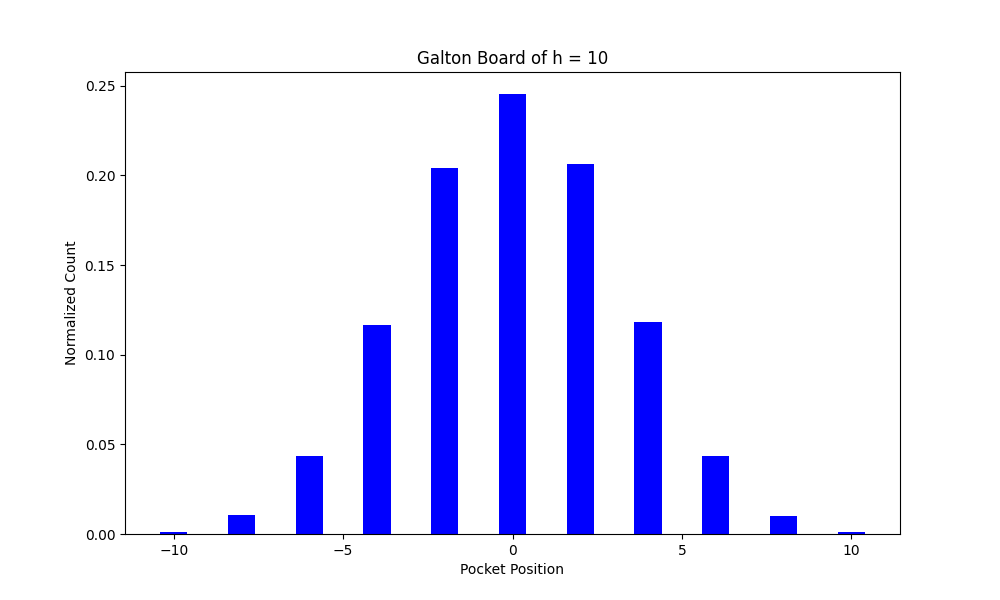
\includegraphics[width=0.75\linewidth]{2d1.png}
     \caption{\\h=10}
\end{center}
\begin{center}
     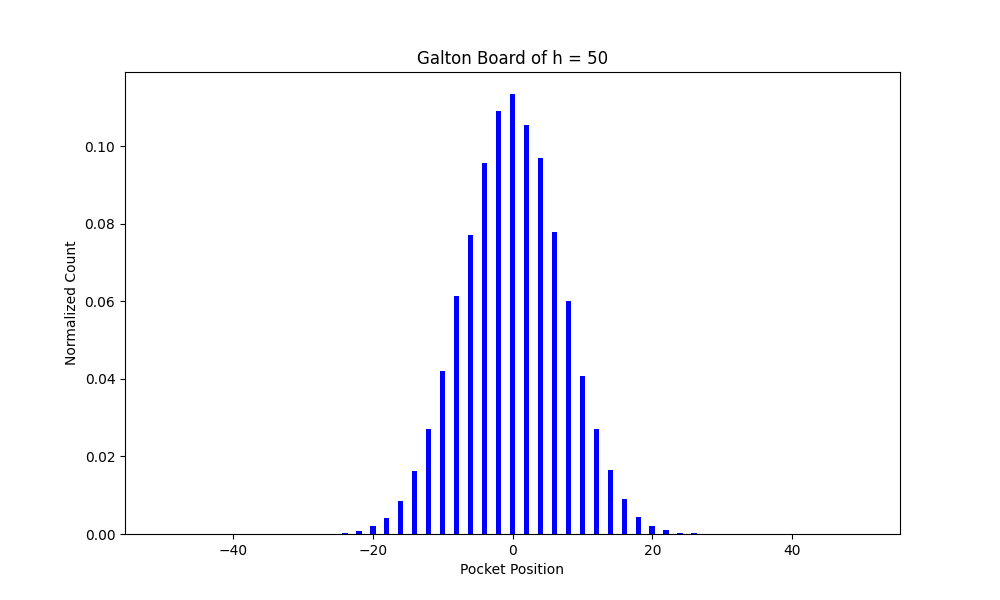
\includegraphics[width=0.75\linewidth]{2d2.png}
     \caption{\\h=50}
\end{center}
\begin{center}
     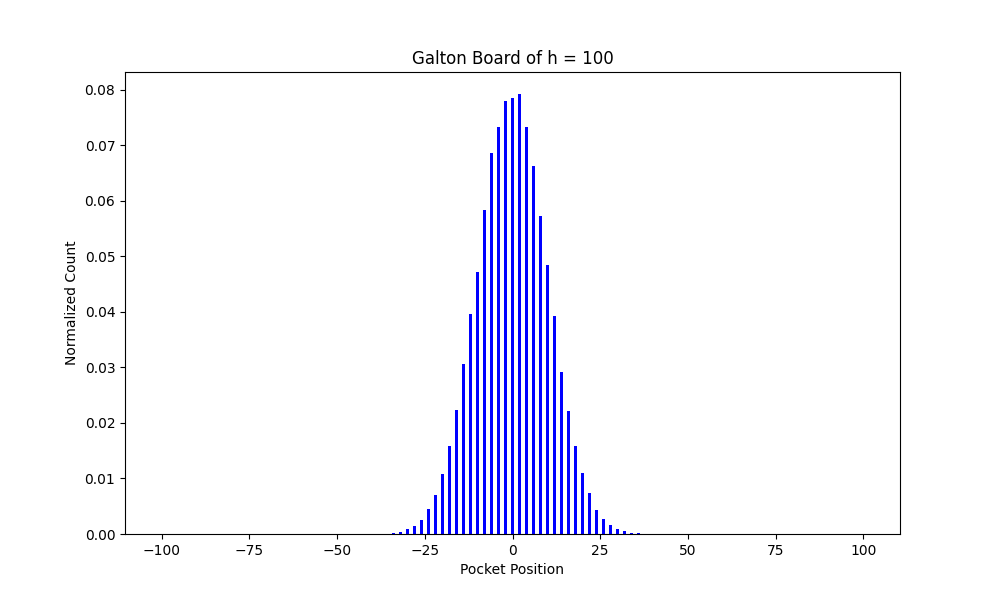
\includegraphics[width=0.75\linewidth]{2d3.png}
     \caption{\\h=100}
\end{center}

The shapes of these histograms closely approach the shape of a gaussian.
\end{solution}

Task E:

\begin{solution}
% To analyze the distribution of the final position \( X \) in the Galton board, we derive a closed-form expression for \( P_h[X = 2i] \), and we show that for large enough \( h \), the distribution approximates a normal distribution \( \mathcal{N}(0, h/2) \).

% ### 1. **Binomial Distribution Interpretation**

Each collision of the ball in a Galton Board has two possible outcomes: moving left or right.Hence, the motion of the ball can be modeled as a series of \( h \) independent Bernoulli trials with parameter $p=\frac{1}{2}$ (as both left and right are equally likely). \\
Now, a series of \( h \) Bernoulli trials can be represented as a binomial distribution with parameters \( h \) and \( p = p_{Bern} = 1/2 \). Let $R \sim Bin(h, 1/2)$ be the random variable representing the number of right moves out of \( h \).\\

If the ball moves to the right \( r \) times out of \( h \), the final position \( X \) can be expressed as:
\[
X = r - (h-r) = 2r-h
\]

Note that since h is even, \( X \) is even and can only take values in \( \{-h, -h+2, \dots, h-2, h\} \).

The probability of landing in a specific pocket corresponding to position \( X = 2i \) is given by:
\[
P(X = 2i) = P(2R-h = 2i) = P(R = i + (h)/2)
\]
Let \( k = h/2 \). From the binomial distribution,

\begin{align*}
P(X = 2i) &= \binom{h}{k+i} \left( \frac{1}{2} \right)^h\\
&= \left( \frac{1}{2} \right)^h \frac{h!}{(k+i)! (k-i)!}\\
\end{align*}

Now, Stirling's approximation for the factorial is $n! \approx \sqrt{2\pi n} \left(\frac{n}{e}\right)^n$.
Assuming that h is very large, and $i<<h$, we can use Stirling's approximation for \( h \), \( k+i \), and \( k-i \):
\begin{align*}
P(X = 2i) &\approx(\frac{1}{2})^h \frac{\sqrt{2\pi h} (\frac{h}{e})^h}{\left(\sqrt{2\pi (k+i)} \left(\frac{k+i}{e}\right)^{k+i}\right)\left(\sqrt{2\pi (k-i)} \left(\frac{k-i}{e}\right)^{k-i}\right)}\\
&= \sqrt{\frac{h}{2\pi (k^2-i^2)}} \frac{h^h}{(h+2i)^{k+i} (h-2i)^{k-i}}\\
&\approx \sqrt{\frac{h}{2 \pi k^2}} \frac{h^h}{{((h+2i)(h-2i))}^{k}} {(\frac{h-2i}{h+2i})}^i\\
&= \sqrt{\frac{1}{\pi k}} {(\frac{1}{1-i^2/k^2})}^{k} {(1- \frac{4i}{h+2i})}^i\\
&\approx \sqrt{\frac{1}{\pi k}} (1+\frac{i^2}{k}) (1- \frac{2i^2}{k})\\
&\approx \sqrt{\frac{1}{\pi k}} (1-\frac{i^2}{k})\\
&\approx \sqrt{\frac{1}{\pi k}} e^{-i^2/k}
\end{align*}

Hence, $P_h[X = 2i] \approx \frac{1}{\sqrt{\pi h}} e^{-\frac{i^2}{h}}= N(0, k/2)$.

This confirms that the distribution of the number of balls in each pocket approaches a normal distribution as \( h \) increases.

\end{solution}

\end{questions}
\end{document}